%----------------------------------------------------------------------------------------
%	PACKAGES AND OTHER DOCUMENT CONFIGURATIONS
%----------------------------------------------------------------------------------------
\documentclass[a4paper,11pt]{article}
\usepackage[a4paper,textwidth=140mm,textheight=245mm]{geometry}
\usepackage[utf8]{inputenc}
\usepackage{listings}
\usepackage{graphicx}
\makeatletter
\renewcommand{\section}{\@startsection
   {section}%                         name
   {1}%                               level
   {0mm}%                             indent
   {-1.5\baselineskip}%               space above header
   {0.5\baselineskip}%                space under header
   {\sffamily\bfseries\upshape\normalsize}}% style
   
\renewcommand{\thesubsection}{\thesection.\alph{subsection}}
\renewcommand{\subsection}{\@startsection
   {subsection}%                      name
   {2}%                               level
   {0mm}%                             indent
   {-0.75\baselineskip}%              space above header
   {0.25\baselineskip}%               space under header
   {\rmfamily\normalfont\slshape\normalsize}}% style
\renewcommand{\subsubsection}{\@startsection
   {subsubsection}%                    name
   {3}%                               level
   {-10mm}%                             indent
   {-0.75\baselineskip}%              space above header
   {0.25\baselineskip}%               space under header
   {\rmfamily\normalfont\slshape\normalsize}}% style
\makeatother
\begin{document}
\begin{titlepage}
\title{TDDC93 Exercises:\\
Requirements}
\author{Martin Söderén\\ marso329@student.liu.se\\900929-1098}
\date{\today}
\maketitle




\vfill % Fill the rest of the page with whitespace

\thispagestyle{empty}

\end{titlepage}
\section{Requirements}
\subsection{Write 2 different use cases with 3 different actors. Draw a use-case diagram for these use-cases and actors. Please remember that the texts for the use cases should not just describe a basic function of the system, such as login. Use standard-UML as shown in the lecture:}
\centerline{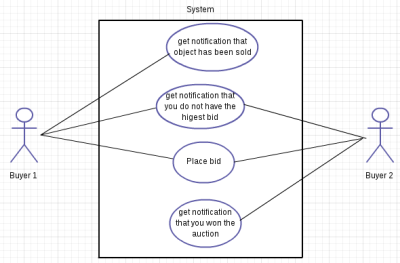
\includegraphics[scale=0.8]{usecase1}}
Description: \newline
Buyer 1 finds an auction with an object that he wants to buy. He places a bid. The same happends to buyer 2 who places a higher bid. Buyer on gets a notification that he does not have the highest bid on the auction. He enters the auctions page again and places a bid that is higher. Now buyer 2 get a notification. This can go on until the time of the auction runs out and by that time Buyer 2 had the highest bid and he gets a notification that he have won tha auction. Buyer 1 gets a notification that the object have been sold to someone else.\newline
\centerline{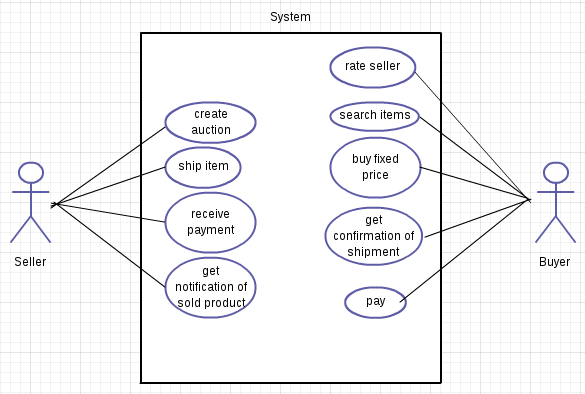
\includegraphics[scale=0.6]{usecase2}}
Description: \newline
The Seller creates an auction. The Buyer finds this auctions by searching through the system and the buys it for the fixed price and makes the payment. The Seller get a notification the the object has been sold and ships it. The Buyer gets a notification that the object has been shipped and when the object is received he can rate the Seller. Then the Seller recevies payment.
\subsection{Write down 5 functional requirements of some part of the system:}
\begin{itemize}
  \item Buyers can bid on offerings
  \item Buyers can search using free-text
  \item Buyers can see the current top categories on the first page
  \item Buyers can rate sellers
  \item Buyers can pay using safe payments system 
\end{itemize}
\subsection{Write down 5 non-functional requirements of the system:}
\begin{itemize}
  \item The system most cost less than 100000\$ to develop
  \item The system must be implemented using PHP
  \item The system must be safe against SQL-injection attacks
  \item The system must be able to handle 100000 users at the same time
  \item The system must be upgradable to handle a million users at the same time 
\end{itemize}
\subsection{Create 5 user stories for some part of the system. Don’t forget to describe which part you are writing about:}
 I'm writing about the part of the system which the buyers will use. 
\begin{itemize}
  \item I as a buyer would like to make safe payments so that nobody will get hold of my credit card information
  \item I as a buyer would like to search all products for sale using free-text so I can find what I am looking for.
  \item I as buyer would like to bid on auctions so I can buy objects.
  \item I as buyer would like to give sellers ratings so I can warn other buyers of bad sellers.
  \item I as a buyer would like to have all the functionality of the webpage in my cellphone so I can buy objects wherever I am.
\end{itemize}

\end{document}